\documentclass[a4paper,12pt]{article}
\usepackage[utf8]{inputenc}
\usepackage{amsmath}
\usepackage{geometry}
\usepackage{fancyhdr}
\usepackage{listings}
\usepackage{xcolor}
\usepackage{graphicx}
\usepackage{float}

% Margins
\geometry{left=15mm, right=15mm, top=25mm, bottom=15mm}

% Header/Footer
\pagestyle{fancy}
\fancyhf{}
\renewcommand{\headrulewidth}{0pt}
\rfoot{Page \thepage}

\fancypagestyle{firstpage}{
    \fancyhf{}
    \lhead{
        \small \textbf{Name:} Mrigaj Shaw \\ 
        \small \textbf{Roll No:} 2024CSB041
    }
    \chead{\LARGE \textbf{Assignment 5}} 
    \rfoot{Page \thepage}
    \renewcommand{\headrulewidth}{1pt}
}

% Code Style
\definecolor{codegreen}{rgb}{0,0.6,0}
\definecolor{codegray}{rgb}{0.5,0.5,0.5}
\definecolor{codepurple}{rgb}{0.58,0,0.82}
\definecolor{backcolour}{rgb}{0.95,0.95,0.92}

\lstdefinestyle{MyCodeStyle}{
    backgroundcolor=\color{backcolour},   
    commentstyle=\color{codegreen},
    keywordstyle=\color{magenta},
    numberstyle=\tiny\color{codegray},
    stringstyle=\color{codepurple},
    basicstyle=\ttfamily\footnotesize,
    breakatwhitespace=false,         
    breaklines=true,                 
    keepspaces=true,                 
    numbers=left,                    
    numbersep=5pt,                  
    showspaces=false,                
    showstringspaces=false,
    showtabs=false,                  
    tabsize=4
}
\lstset{style=MyCodeStyle}

\begin{document}
\thispagestyle{firstpage}

% --- Problem1 ---
\section*{Problem 1}
\textbf{Problem Statement:} Let $S = \{0, 1, 2, \dots, n - 1\}$ be a set of $n$ distinct elements. Initially, each element forms its own separate set, so the collection consists of $n$ disjoint singleton sets. This initial configuration is represented using a parent array $P$ of size $n$, where $P[i] = i$ for all $0 \le i \le n - 1$, and a rank array $R$, where $R[i] = 0$ for all $0 \le i \le n - 1$.

Design and implement an efficient Disjoint Set (Union--Find) data structure that supports two fundamental operations: \texttt{Find(x)}, which returns the representative (root) of the set containing element $x$, and \texttt{Union(x, y)}, which merges the two sets containing elements $x$ and $y$. To improve efficiency, apply path compression during the \texttt{Find} operation so that each visited node directly points to the root, and apply union by rank during the \texttt{Union} operation so that the tree with smaller height is attached under the tree with larger height, thereby keeping the tree shallow.
\subsection*{Code}
\lstinputlisting[language=C]{Problem1/DisjointSet.c}
\subsection*{Output}
\begin{figure}[H]
    \centering
    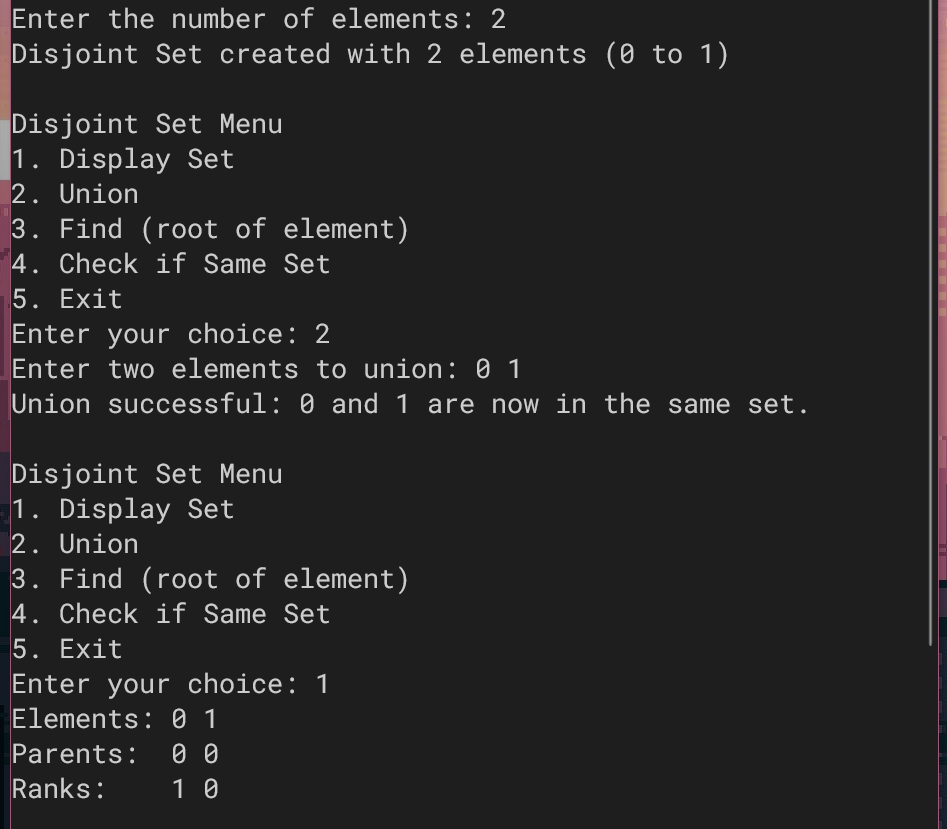
\includegraphics[width=0.9\textwidth]{Problem1/Problem1.png}
\end{figure}
\subsection*{Inference}

The following conclusions can be drawn from the foundational implementation of the Disjoint Set Union (DSU) data structure:

\begin{enumerate}
    \item \textbf{Data Structure Functionality}:
    \begin{itemize}
        \item The implementation successfully manages a collection of elements partitioned into non-overlapping (disjoint) subsets, providing a robust mathematical foundation for dynamic connectivity problems.
    \end{itemize}

    \item \textbf{Operation Mechanics, Path Compression, and Amortized Time}:
    \begin{itemize}
        \item \textbf{Find and Path Compression}: The \texttt{find} operation locates the root representative of a set. To drastically optimize this, a technique called \textit{path compression} is employed. During a \texttt{find} traversal, every node visited along the path is updated to point directly to the root. This permanently flattens the tree structure, ensuring subsequent accesses are instantaneous.
        \item \textbf{Union and Amortized Complexity}: The \texttt{union(a, b)} function relies entirely on the \texttt{find} operation to locate the two roots before linking them. By combining path compression with union by size/rank, the cost of these operations drops to $O(\alpha(n))$, where $\alpha(n)$ is the Inverse Ackermann function. Because $\alpha(n) \le 4$ for any computationally feasible input, the \textbf{amortized time complexity} is practically $O(1)$. \textit{Amortized time} means that while a single operation might occasionally take longer (e.g., the first deep path compression), the average time per operation over a sequence is mathematically guaranteed to be constant.
    \end{itemize}

    \item \textbf{Space Allocation}: 
    \begin{itemize}
        \item The structure requires $O(n)$ auxiliary space to store the \texttt{parent} array (and optionally the \texttt{rank} or \texttt{size} arrays) to maintain the state of the $n$ elements.
    \end{itemize}
\end{enumerate}

\newpage

% --- Problem2 ---
\section*{Problem 2}
\textbf{Problem Statement:} In a large school campus, thousands of students dynamically form different friend groups, where new friendships are created daily and teachers frequently need to verify whether two students belong to the same group. Initially, each student forms an independent group. As interactions increase, multiple groups gradually merge, and it becomes essential to efficiently manage these dynamic group connections.

Given $n$ students and $m$ randomly generated friendship operations, design and implement an optimized \textbf{Disjoint Set (Union--Find)} data structure using \textbf{dynamic arrays}, which supports two fundamental operations:                                              

\begin{itemize}
    \item \texttt{Union(x, y)}: Merges the sets containing students $x$ and $y$.
    \item \texttt{Find(x)}: Returns the representative (leader) of the set containing student $x$.
\end{itemize}

Let the initial parent array be defined as:
$$P[i] = i, \quad \text{for all } 0 \le i \le n - 1$$

To enhance performance, apply \textbf{path compression} during the \texttt{Find} operation and \textbf{union by rank} during the \texttt{Union} operation. The system must efficiently process all $m$ operations, ensuring fast connectivity queries even for large values of $n$ and $m$.
\subsection*{Code}
\lstinputlisting[language=C]{Problem2/friendshipOperations.c}
\subsection*{Output}
\begin{figure}[H]
    \centering
    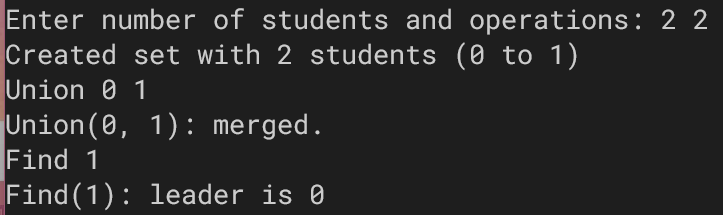
\includegraphics[width=0.9\textwidth]{Problem2/Problem2.png}
\end{figure}
\subsection*{Inference}

Based on the application of DSU to model a social network, the following insights can be highlighted:

\begin{enumerate}
    \item \textbf{Graph Modeling \& Algorithmic Mapping}:
    \begin{itemize}
        \item The problem effectively translates a real-world social network into an undirected graph. Establishing a new friendship maps directly to the \texttt{union} operation, seamlessly merging two separate friend groups into a single extended network.
        \item Checking if two individuals belong to the same extended friend circle utilizes the \texttt{find} operation to verify if they share the identical root representative.
    \end{itemize}

    \item \textbf{Scalability and Application}:
    \begin{itemize}
        \item Because the underlying operations operate in amortized constant time (as established in Problem 1), this approach is perfectly suited for dynamic social networks. It provides real-time query responses without the immense computational overhead of performing a full graph traversal (like BFS or DFS) for every single query, keeping operations strictly $O(1)$ on average and space strictly $O(n)$.
    \end{itemize}
\end{enumerate}

\vspace{0.5em}
\noindent \textbf{Note:} \texttt{DisjointSetUnion.h} includes the exact same logic and functions implemented and analyzed in Problem 1.

\newpage

% --- Problem3 ---

\section*{Problem 3}
\textbf{Problem Statement:} A city contains $N$ buildings, initially all isolated, which can be mathematically modeled as $N$ disjoint singleton sets, where the parent array is initialized as
$$P[i] = i, \quad \text{for all } 0 \le i \le N - 1.$$

Over time, $M$ road construction operations are performed, where each operation connects two buildings $(u, v)$, with $0 \le u, v \le N - 1$. To efficiently manage these dynamic connections, design a \textbf{Disjoint Set (Union--Find)} data structure supporting two operations: \textit{Union(u, v)}, which merges the sets containing $u$ and $v$, and \textit{Find(x)}, which returns the representative (leader) of the set containing $x$. After each union operation, the system must verify whether the entire city has become fully connected, which mathematically implies that all buildings belong to a single connected component, i.e., there exists a unique representative $r$ such that
$$\text{Find}(i) = r, \quad \text{for all } 0 \le i \le N - 1.$$

\subsection*{Code}
\lstinputlisting[language=C]{Problem3/roadConstruction.c}
\subsection*{Output}
\begin{figure}[H]
    \centering
    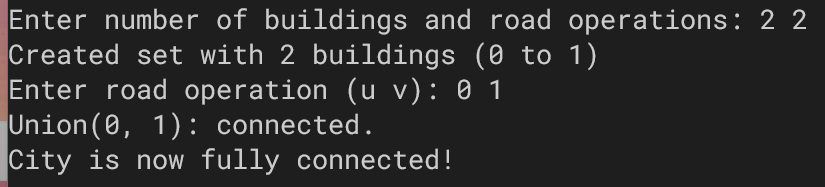
\includegraphics[width=0.9\textwidth]{Problem3/Problem3.png}
\end{figure}

\subsection*{Inference}

The application of DSU for infrastructural planning (road construction) yields the following technical insights:

\begin{enumerate}
    \item \textbf{Connectivity Verification \& Universal Root Matching}:
    \begin{itemize}
        \item The DSU explicitly verifies the progressive connectivity of the road network by evaluating the collective root state of all buildings.
        \item After each road construction (\texttt{union} operation), the algorithm isolates the representative root of the first building (building 0) and iterates through all remaining buildings. If every building returns the exact same root, it mathematically proves the entire city has merged into a single connected component.
    \end{itemize}

    \item \textbf{Infrastructural Suitability}:
    \begin{itemize}
        \item Evaluating $M$ proposed roads connecting $N$ cities requires minimal overhead. Because the operations utilize path compression (as detailed in Problem 1), both the \texttt{union} step and the sequential \texttt{find} checks during the connectivity verification happen in amortized constant time. This iterative validation ensures absolute accuracy and demonstrates the foundational logic required for spanning tree validations.
    \end{itemize}
\end{enumerate}

\vspace{0.5em}
\noindent \textbf{Note:} \texttt{DisjointSetUnion.h} includes the exact same logic and functions implemented and analyzed in Problem 1.

\end{document}